\section{Arrow-based conditions}
\slabel{ab-conditions}

In this section we recall the standard notion of nested condition from~\cite{Rensink-FOL}, using notations that will make the connection with the variation proposed in this paper as straightforward as possible. Here and in the remainder of the paper, we will mostly omit the term ``nested'' and just refer to \emph{conditions}; however, to distinguish between variations upon this theme, we will refer to the standard notion of nested conditions as \emph{arrow-based}.

Along the paper examples and intuitions will be based on $\cat{Graph}$, the category of directed, edge-labelled multigraphs. Let us introduce the formal definition, as well as some constructions and operations on graphs we will need later.

\begin{definition}[Category of Graphs]\label{def:graph-and-morphism}
  A \emph{graph}~$G = (V_G,E_G,s_G,t_G,\ell_G)$ has sets~$V_G$ of nodes and~$E_G$ of edges, along with source and target functions~$s_G,t_G\of E_G\to V_G$, and an edge-labeling function $\ell_G\of E_G \to \Lab$.\footnote{Without loss of generality we assume $V_G \cap E_G= \varnothing$.}
  A \emph{graph morphism}~$f:G\to H$ is a pair of functions~$f = (f_V\of V_G\to V_H, f_E\of E_G\to E_H)$ that preserve incidence (that is, $s_G; f_V = f_E;s_H$ and $t_G; f_V = f_E ; t_H$) and labels ($f_E;\ell_H = \ell_G$).
  Graphs and graph morphisms determine the category of graphs~$\cat{Graph}$.

  Given a set $X$, we denote by $\disc{X} = (X,\varnothing,\varnothing,\varnothing,\varnothing)$ the \emph{discrete graph} having $X$ as nodes; thus $\disc{\varnothing}$ denotes the empty graph. Given a function $f\of X \to Y$ and a subset $X' \subseteq X$, by $f\restr X'\of X' \to Y$ we denote the obvious restriction. Graph $G$ is a \emph{subgraph} of $H$, written $G \subseteq H$, if $V_G \subseteq V_H$, $E_G \subseteq E_H$, $s_G = s_H\restr E_G$, $t_G = t_H\restr E_G$ and $\ell_G = \ell_H\restr E_G$. If $g \of H \to K$ is a graph morphism and $G \subseteq H$, then $g \restr G \of G \to K$ is its restriction defined componentwise for nodes and edges.  


  Graphs $G$ and $H$ are \emph{disjoint} if $V_G \cap V_H = \varnothing = E_G \cap E_H$. In this case their \emph{(disjoint) union} is the graph $G \uplus H$, defined in the expected way. Given morphisms $g\of G \to K$ and $h \of H \to K$, if $G$ and $H$ are disjoint we denote by $[g,h]\of G\uplus H \to K$ the morphism defined as $[g,h](x) = g(x)$ if $x \in G$, and $[g,h](x) = h(x)$ if $x \in H$.\footnote{When not ambiguous we may omit some subscripts and use a graph name $G$ to denote the set of its items $V_G \cup E_G$.}
\end{definition}

Referring to a graph, we often write $\oneedgewithlab{x}{e}{a}{y}$ to say that edge $e$ is such that $\ell(e)= \la$, $s(e) = x$ and $t(e) = y$, and $\oneedge{x}{a}{y}$ if there is such an edge.

\medskip

Though examples will be based on $\cat{Graph}$, formal definitions and results will be phrased in terms of objects and arrows of a generic category $\bC$ that we assume to be a \emph{presheaf topos}, i.e., a category of contravariant functors from a small category \cat{S} to \cat{Set}, thus \cat{C} $= [\op{\cat{S}} \to \cat{Set}]$. Several categories of graphs and hypergraphs are presheaf toposes: for example, directed unlabeled graphs are obtained with \cat{S} the free category generated by $\mygraph{
  \node (1) {$\bullet$};
  \node (2) [right=of 1] {$\bullet$};
  \path (1) edge[bend left=20,->] (2)
        (1) edge[bend right=20,->] (2);
}$.\todo{Maybe say what $\Graph$ is as a presheaf topos?} Furthermore, presheaf toposes are closed under the construction of slice and functor categories, thus they include labeled/typed (hyper)graphs (see Sec.~5 of~\cite{AzziCR19}). We will denote the collection of objects of a category $\cat{C}$ by $|\cat{C}|$, and for $A,B \in |\cat{C}|$ we denote by $\cat{C}(A,B)$ the (hom)set of arrows from $A$ to $B$.  

Assuming that \cat{C} is a presheaf topos ensures several properties we need in the constructions of this paper: in particular, that all limits and colimits exist (and can be computed pointwise), and also that epis are stable under pullback. Furthermore, \cat{C} is \emph{adhesive}~\cite{ls:adhesive-journal}, enjoying several properties exploited in the algebraic theory of graph rewriting, where the results of this paper have potential interesting applications.\footnote{Note that requiring \cat{C} to be just adhesive would not suffice: for example, we need arbitrary pushouts, while adhesivity only guarantees pushouts along monos.}

\medskip\noindent
Arrow-based conditions are inductively defined as follows:

\begin{definition}[arrow-based condition]\dlabel{ab-condition}
  Let $R$ be an object of $\bC$. $\AC R$ (the set of \emph{arrow-based conditions} over $R$) and $\AB R$ (the set of \emph{arrow-based branches} over $R$) are the smallest sets such that
  \begin{itemize}
  \item $c\in \AC R$ if $c=(R,p_1\ccdots p_w)$ is a pair with $p_i\in \AB R$ for all $1\leq i\leq w$, where $w \geq 0$;
  \item $p\in \AB R$ if $p=(a,c)$ where $a: R\to P$ is an arrow of $\bC$ and $c\in \AC P$.
  \end{itemize}
\end{definition}
%
We regularly abbreviate ``arrow-based" to ``ab". We call $R$ the \emph{root} of an ab-condition or ab-branch, and $P$ the \emph{pattern} of an ab-branch (which is simultaneously the root of its subconditon). \fcite{ab-condition} provides a visualisation of an ab-condition $c$. We use $b,c$ to range over ab-conditions and $p,q$ to range over ab-branches. We use $|c|=w$ to denote the width of an ab-condition $c$, $R^c$ to denote its root, and $p^c_i=(a^c_i,c_i)$ its $i$-th branch. Finally, we use $P^c_i$ ($=R^{c_i}$) for the pattern of branch $p^c_i$. In all these cases, we may omit the superscript $c$ if it is clear from the context.
%
\begin{figure}[t]
\centering
\subcaptionbox
  {Condition $c=(R,p_1\ccdots p_w)$, with $p_i=(a_i,c_i)$ for $1\leq i\leq w$
   \flabel{ab-condition}}
  [.45\textwidth]
  {\begin{tikzpicture}
  \node (top) {$R_C$};
  \node (C1) [triangle,below left=of top] {$c_1$};
  \node [below=of top] {$\cdots$};
  \node (Cn) [triangle,below right=of top] {$c_n$};

  \path (C1.north) edge[<-] node[above left] {$r_1$} (top)
        (Cn.north) edge[<-] node[above right] {$r_n$} (top);
\end{tikzpicture}
}
\quad
\subcaptionbox
  {$g\sat c$, with responsible branch $p_i=(a_i,c_i)$ and witness $h$ such that $g=a_i;h$
   \flabel{ab-satisfaction}}
  [.5\textwidth]
  {\begin{tikzpicture}[on grid]
  \node (R) {$R_c$};
  \node (P1) [below left=of R] {};
  \node [below left=.8 and .4 of R] {$\cdots$};
  \node (Pi) [below=1.8 of R] {$P^i$};
  \node [below right=.8 and .4 of R] {$\cdots$};
  \node (Pn) [below right=of R] {};
  \node (ci) [triangle,below=.15 of Pi.center] {$c_i$};
  \node (G) [right=2 of R] {$G$};

  \path (R) edge [->] (P1)
        (R) edge [->] (Pn)
		(R) edge[->] node[above] {$g$} (G)
        (R) edge[->] node[left,near end] {$r_p$} (Pi)
        (Pi) edge[->,bend right] node[pos=0.2,below right] (h) {$h$} (G)
        (h) edge[draw=none] node[sloped,allow upside down] {$\nsat$} (ci);
\end{tikzpicture}
}
\caption{Visualisations for arrow-based conditions}
\end{figure}

Note that, as a consequence of the inductive nature of \dcite{ab-condition}, every ab-condition has a finite \emph{depth} $\depth(c)$, defined as $0$ if $|c|=0$ and $1+\max_{1\leq i\leq |c|} \depth(c_i)$ otherwise. The depth will provide a basis for inductive proofs.

\begin{example}\exlabel{ab-conditions}
\fcite{ab-conditions} shows the graphical representation of three arrow-based conditions, rooted in the discrete one-node graph \inline{\onenode x}. The leftmost one, $c_1 \in \AC{\inline{\onenode x}}$, is defined according to \dcite{ab-condition} as 

$\begin{array}{ll}
c_1 = (\inline{\onenode x}, (f,c_{11})) & c_{11} = (\inline{\oneloopleft{x}{b}}, (g,c_{111})(h,c_{112}))\\
c_{111} = (\inline{\looponeedge{x}{b}{a}{y}}, \epsilon) & c_{112} = (\inline{\looponeedge{x}{b}{c}{y}}, \epsilon)
\end{array}$

\noindent
For the depths,  $\depth(c_{111}) = \depth(c_{112}) = 0$, $\depth(c_{11}) = 1$ and $\depth(c_1) = 2$.


Anticipating the correspondence with FOL discussed later, assuming that we already know the image of $x$ in a graph, the three conditions enjoy the following:
\begin{itemize}
\item $c_1$ is equivalent to $\lb(x,x)\wedge \neg \exists y\st(\la(x,y)\vee \lc(x,y))$
\item $c_2$ is equivalent to $\exists y\st \lb(x,y) \wedge \neg \la(y,y)\wedge \neg \exists z\st \lc(y,z)$ 
\item $c_3$ is equivalent to $\la(x,x)\vee (\exists y\st \lb(x,y) \wedge (\forall v,z\st \lc(y,v)\wedge \lc(y,z) \rightarrow v=z))$
\end{itemize}
%
Note that we have used variable names to represent nodes, to make the connection to the corresponding FOL properties more understandable. The morphisms are in all cases implied by the graph structure and variable names.
\qed
\end{example}
%
\begin{figure}[t]
\centering
\begin{tikzpicture}[on grid]
  \node[graph] (10) {\onenode{x}};
  \node[left=0 of 10.west,inner sep=0] {$c_1$};
  \node[graph,below=of 10] (11) {\oneedge{x}{b}{y}}; 
  \node[left=0 of 11.west,inner sep=0] {$c_{11}$};
  \node[graph,below left=1 and 1.1 of 11] (111) {\oneedgeloop{x}{b}{y}{a}};
  \node[above right=0 of 111.north west,inner sep=1] {$c_{111}$};
  \node[graph,below right=1 and 1.1 of 11] (112) {\twoedge{x}{b}{y}{c}{z}};
  \node[above left=0 of 112.north east,inner sep=1] {$c_{112}$};
  
  \path (10) edge[->] (11)
        (11) edge[->] (111)
        (11) edge[->] (112);
  
  \node[graph,right=3.5 of 10] (20) {\onenode{x}};
  \node[left=0 of 20.west,inner sep=0] {$c_2$};
  \node[graph,below left=of 20] (21) {\oneloop{x}{a}}; 
  \node[left=0 of 21.west,inner sep=0] {$c_{21}$};
  \node[graph,below right=of 20] (22) {\oneedge{x}{b}{y}}; 
  \node[right=0 of 22.east,inner sep=0] {$c_{21}$};
  \node[graph,below=1.2 of 22] (221) {\onetwoedge{x}{b}{y}{c}{v}{c}{z}}; 
  \node[above left=0 of 221.north east,inner sep=1] {$c_{221}$};
  \node[graph,below=1.2 of 221] (2211) {\twoedge{x}{b}{y}{c}{z}}; 
  \node[above left=0 of 2211.north east,inner sep=1] {$c_{2211}$};

  \path (20) edge[->] (21)
        (20) edge[->] (22)
		(22) edge[->] (221)
		(221) edge[->] node[left] {\mapping{v&z}} (2211);

  \node[graph] [right=4.5 of 20] (30) {\onenode{x}};
  \node[left=0 of 30.west,inner sep=0] {$c_3$};
  \node[graph,below=of 30] (31) {\oneloopleft{x}{b}}; 
  \node[left=0 of 31.west,inner sep=0] {$c_{31}$};
  \node[graph,below left=1 and 1.1 of 31] (311) {\looponeedge{x}{b}{a}{y}};
  \node[above right=0 of 311.north west,inner sep=1] {$c_{311}$};
  \node[graph,below right=1 and 1.1 of 31] (312) {\looponeedge{x}{b}{c}{y}};
  \node[above left=0 of 312.north east,inner sep=1] {$c_{312}$};
  
  \path (30) edge[->] (31)
        (31) edge[->] (311)
        (31) edge[->] (312);
\end{tikzpicture}


\caption{Examples of arrow-based conditions (see \excite{ab-conditions})}
\flabel{ab-conditions}
\end{figure}


\paragraph{Shifting and prefixing ab-conditions}
We introduce two basic operations over ab-conditions that allow one to change the root by exploiting arrows from or to the root. 
Given an ab-condition $c \in \AC{R}$ and an arrow $g\of S \to R$, we can \emph{precompose} $c$ with $g$ obtaining a condition $\bshift{c}{g} \in \AC{S}$. Dually, given an arrow $f\of R \to Q$, we can \emph{shift} $c$ along $f$ by exploiting the existence of pushouts in $\cat{C}$, obtaining a condition $\shift{c}{f} \in \AC{Q}$.

For the components of the pushout of two arrows $f\of R \to Q$ and $a \of R \to P$ we will use the notation illustrated in the following diagram, assuming that $( P\tdarr Q, f\tdarr a, a\tdarr f)$ is a concretely chosen pushout of $f$ and $a$ (which is defined up to isomorphism).

\begin{equation}\label{eq:pushout}
    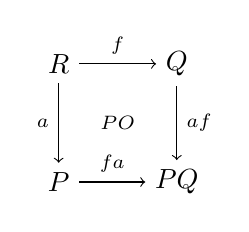
\begin{tikzpicture}[auto,node distance = 1.5cm]
      \node (R) {$R$};
      \node (Q) [right of=R] {$Q$}
      edge [<-] node[auto,swap] {$\scriptstyle{f}$}  (R);
      \node (P) [below of=R] {$P$}
      edge [<-] node[auto] {$\scriptstyle{a}$}  (R);
      \node (PO) [below of=Q] {$P\tdarr Q$}
edge [<-] node[auto,swap] {$\scriptstyle{a\tdarr f}$}  (Q)
edge [<-] node[auto,swap] {$\scriptstyle{f\tdarr a}$}  (P); 
\draw (.75,-.75) node {$\scriptstyle{PO}$};
    \end{tikzpicture}
  \end{equation} 

\begin{definition}[precomposition and shift of ab-conditions]
  \label{def:shift}
Let   $c=(R,p_1\ccdots p_w)$ be an ab-condition in $\AC R$, with $p_i = (a_i\of R\to P_i,c_i)$ for $i\in [1,w]$, where $c_i \in \AC{P_i}$.\todo{AC: add figures}
\begin{itemize}
\item 
Let $g\of S \to R$ be an arrow in $\cat{C}$. The \emph{precomposition of $c$ with $g$} is the condition $\bshift{c}{g} \in \AC{S}$ defined as $\bshift{c}{g} = (S,p'_1\ccdots p'_w)$, where $p'_i = (g;a_i\of S\to P_i,c_i)$ for $i\in [1,w]$.
\item
Let $f\of R \to Q$ be an arrow. The \emph{shift of $c$ along $f$} is the condition $\shift{c}{f} \in \AC{Q}$ defined as  $\shift{c}{f} = (Q, p''_1\ccdots p''_w)$, where $p''_i = (a_i \tdarr f\of Q \to P_i \tdarr Q, \shift{c_i} {(f\tdarr {a_i})})$ for $i\in [1,w]$.
\end{itemize}

\end{definition}

Note that \emph{precomposing} an ab-codition with an arrow only affects the top-level branches, and the subconditions are preseved. Instead \emph{shifting} a condition along an arrow affects all subconditions, which are recursively shifted along the corresponding pushout arrows. 

\subsection{Satisfaction}

A condition expresses a property of arrows from its root to arbitrary objects. This is operationalised through the notion of \emph{satisfaction}.

\begin{definition}[satisfaction of arrow-based conditions]\dlabel{ab-satisfaction}
  Let $c$ be an ab-condition over $R$ and $g:R\to G$ an arrow from $c$'s root to some object $G$. We say that \emph{$g$ satisfies $c$}, denoted $g\sat c$, if there is a branch $p_i=(a_i,c_i)$ of $c$ and an arrow $h:P_i\to G$ such that
  \begin{enumerate}
  \item $g=a_i;h$ and
  \item $h\nsat c_i$.
  \end{enumerate}
\end{definition}
%
If $g\sat c$, we also say that $g$ is a \emph{model} for $c$. We call $p_i$ the \emph{responsible branch} and $h$ the \emph{witness} for $g\sat c$. Pictorially, $g\sat c$ with responsible branch $p_i$ and witness $h$ can be visualised as in \fcite{ab-satisfaction}.

Based on the notion of satisfaction, for ab-conditions $b$ and $c$ (over the same root) we  define \emph{semantic entailment} $b\entails c$ and \emph{semantic equivalence} $b\equiv c$:
%
\begin{align*}
b \entails c & \text{ if for all arrows $g$: } g\sat b \text{ implies } g\sat c \\
b \equiv c & \text{ if for all arrows $g$: } g\sat b \text{ if and only if } g\sat c \enspace. 
\end{align*}


\begin{example}\exlabel{ab-satisfaction}
Let us consider some models for the ab-conditions in \fcite{ab-conditions}.
\begin{itemize}[topsep=0pt]
\item Let $G_1=\myinlinegraph{
\node (1) {$\bullet$};
\node (2) [right=of 1] {$\bullet$};
\path (1) edge[bend left=20,->] node[near start,above] {\lb} (2)
      (2) edge[bend left=20,->] node[near start,below] {\lb} (1)
	  (1) edge[loop left,->] node[left] {\lc} (1);
}$
and let $g$ be the morphism from the one-node discrete graph \inline{\onenode x} to the left-hand node of $G_1$. It is clear that $g\nsat c_1$ because there is no witness for $c_{11}$ ($G_1$ does not have the required $\lb$-loop). Instead, we have $g\sat c_2$: the witness $h$ (for $c_{21}$) maps $y$ to the right-hand node of $G_1$; and $h$ does not satisfy the subconditions of $c_{21}$ because it cannot be extended with either the $\la$-loop specified by $c_{211}$ or the outgoing $\lc$-edge specified by $c_{212}$. Similarly, $g\sat c_3$.

\item Let $G_2=\myinlinegraph{
\node (1) {$\bullet$};
\node (2) [right=of 1] {$\bullet$};
\node (3) [right=of 2] {$\bullet$};
\path (1) edge[bend left=20,->] node[near start,above] {\lb} (2)
      (2) edge[bend left=20,->] node[near start,below] {\lb} (1)
	  (1) edge[loop left,->] node[left] {\la} (1)
      (2) edge[->] node[above] {\lc} (3);
	  }$
and let $g,g',g''$ be the morphisms from \inline{\onenode x} to $G_2$ mapping \inline{\onenode x} to the left, mid and right node of $G_2$, respectively. None of these models satisfy $c_1$, for the same reason as above. Moreover, none satisfy $c_2$: though $g$ and $g'$ have witnesses for $c_{21}$, these are ruled out by either $c_{212}$ (in the case of $g$) or $c_{211}$ (in the case of $g'$); $g''$ not even has a witness for $c_{21}$. Instead, both $g\sat c_3$ (in fact there are two distinct witnesses, one for $c_{31}$ and one for $c_{32}$) and $g'\sat c_3$ (due to $c_{32}$); but again $g''\nsat c_3$.

\item If $G_3=\inline{\oneloopleft \bullet b}$, then the only morphism $g$ from \inline{\onenode x} to $G_3$ has $g\sat c_1$, $g\sat c_2$ and $g\sat c_3$. 
\end{itemize}
In general, it can be checked that every model of $c_1$ is also a model of $c_2$ and every model of $c_2$ is a model of $c_3$, thus $c_1\entails c_2$ and $c_2 \entails c_3$. On the other hand, $c_2\nsat c_1$ as shown by $g:\inline{\onenode x}\to G_1$, and $c_3 \nsat c_2$ as shown by $g:\inline{\onenode x}\to G_2$.\qed
\end{example}

Shifting a condition along an arrow preserves the models prefixed with such arrow, and precomposing a condition with an arrow preserves the models, and it reflects them if the arrow is epi.

\begin{proposition}[Satisfaction is invariant w.r.t.~shift and precomposition with epis]
  \label{pr:shiftSat}
  \begin{enumerate}
    \item
  Let $c \in \AC R$ and $f\of R \to Q$. Then $f;m \sat c$ iff $m \sat \shift{c}{f}$.
  \item   
  Let $c \in \AC R$ and $g\of S \to R$. Then  $m \sat c$ implies $g;m \sat \bshift{c}{g}$, and if $g$ is epi also the converse holds.
  \end{enumerate}
\end{proposition}

\begin{proof}[]
\textbf{(1)}\hspace{1ex} We proceed by induction on the depth of $c$, noting that shift preserves the depth. If $\depth(c) = 0$ then $c = (R, \epsilon)$ and $\shift{c}{f} = (Q,\epsilon)$; thus for every $m \of Q \to G$ we have $f;m \not \sat c$ and $m \not \sat \shift{c}{f}$. Now let $\depth(c) = n > 0$ and assume that the statement holds for all conditions with depth smaller than $n$.\\
 \textbf{($\Rightarrow$)} Let $m\of Q \to G$ and assume that $f;m \sat c$, meaning that there is a branch $p_i = (a_i\of R \to P_i, c_i)$ of $c$ with $i \in [1,w]$ and an $h: P_i \to G$ such that $(\dagger)\ a_i ; h = f;m$ and $(\ddagger)\ h \not \sat c_i$. To show that $m \sat \shift{c}{f}$, we can consider the branch $(a_i\tdarr f\of Q \to  P_i \tdarr Q, \shift{c_i}{(f\tdarr a_i)})$ of $\shift{c}{f}$, and as witness the arrow $h'\of P_i \tdarr Q \to G$ induced by the universal property of the pushout because of $(\dagger)$. In fact, we have $a_i\tdarr f;h' = m$ by the pushout properties, while $h' \not \sat \shift{c_i}{(f\tdarr a_i)}$ holds by contradiction. Indeed, by induction hypothesis (since $\depth(c_i) < n$) we have $h' \sat \shift{c_i}{(f\tdarr a_i)} \iff f\tdarr a_i ; h' \sat c_i$ which contradicts $(\ddagger)$ because $f\tdarr a_i ; h' = h$ by the pushout properties. \\ 
 \textbf{($\Leftarrow$)} Assume that $m \sat \shift{c}{f}$. Thus there is a branch  
$(a_i\tdarr f\of Q \to  P_i \tdarr Q, \shift{c_i}{(f\tdarr a_i)})$ of $\shift{c}{f}$ and an $h'\of P_i \tdarr Q \to G$ such that $a_i\tdarr f;h' = m$ and $(*)\ h' \not \sat \shift{c_i}{(f\tdarr a_i)}$. We show that $f;m \sat c$ with responsible branch $(a_i\of R \to P_i,c_i)$ and witness  $(\ddagger)\ h \stackrel{\mathit{def}}{=}f\tdarr a_i ; h'$. In fact $a_i; h = a_i; f\tdarr a_i ; h' = f; a_i\tdarr f; h' = f ; m$. Moreover, by induction hypothesis we can assume that $f \tdarr a_i; h' \sat c_i \iff h' \sat \shift{c_i}{(f \tdarr a_i)}$, therefore by $(*)$ and $(\ddagger)$ we conclude that $h \not \sat c_i$.     

\medskip
\noindent
\textbf{(2)}\hspace{1ex}
Spelling out the definitions, it is obvious that if $(a_i, c_i)$ is a responsible branch for $m \sat c$ with witness $h\of P_i \to G$, then $(g;a_i,c_i)$ is a responsible branch for $g;m \sat  \bshift{c}{g}$, with exactly the same witness. In fact $a_i; h = m$ implies $g;a_i ; h = g ; m$. If $g$ is epi also the converse is true. \qed
\end{proof}
